%----- do not modify this first block,

\documentclass[sigconf,review,nonacm]{acmart}

%--- edit from here
\usepackage{blindtext} % package just required to create the filler text
\usepackage{algorithm} 
\usepackage{algpseudocode} 

\begin{document}
\title[Hybrid SMS-EMOA]{Hybridisation of SMS-EMOA with Regression Models}
\author{740036129}

%% Short summary of the report
\begin{abstract}
 \blindtext 

 \textbf{key-terms:}
    \textbf{HVC} Hypervolume Contribution,
    \textbf{SMS-EMOA}
\end{abstract}

%% builds the first part of the formatted document.
\maketitle

\section{Introduction}

A key distinction to make is between Hypervolume and HVC these are linked but HVC builds upon the concept of hypervolume and while using it allows us to distinguish between solutions/individuals that do not contribute much to the whole Hypervolume as a whole. 

When talking about hypervolume when we really mean area for the \textit{ZDT} sets as they use a 2 dimensional objective spaces. TODO: FINISH THIS LINE 

 \blindtext 
 \blindtext 

introduction text goes here 

This whole paper is written with the assumption that hypervolume calculations are computationally expensive. 

\balance

\section{Numerical experiments}

This sections is divided into two major subsections. The first discussing the implemented hybridisation of SMS-EMOA \ref{hybrid}, The second covering default behaviour of SMS-EMOA and the comparison metrics that are utilised and discussed throughout this paper. 

\subsection{Hybridisation of SMS-EMOA}
\label{hybrid}

In SMS-EMOA works based on the \textit{hypervolume} indicator. However it does not actually calculate the actual hypervolume as a whole, instead it calculates the HVC as a part of choosing what parts of the population survives in any given generation. As such the survival function is parsed fronts and returns a number representing an individual's contribution to the population as a whole, this is what the regression model will be used to predict. \\

\noindent As such the regression model(s) do not directly interact with the decision variables instead models the contribution of a given individual on the objective space. 
It would be great if we could parse in a model that replaces HVC that knows the objective landscape before we start optimising, and yes with the \textit{test problems} this can be done but in real situations this is \textit{not always known} as such a hybrid approach is needed where a proportion of the time it is working based on actual HVC calculations and the remaining time it is working based upon a model predicting these HVCs. Here we found that roughly a 50:50 split flipping between prediction and actual calculations every 10 fronts. \\
It was found that working with a flip rate of less than 10 fronts would mean that the model impede convergence towards a diverse set of solutions, this would often cause large gaps or cover only one section of the Pareto front in all the test sets. 

\begin{algorithm}
	\caption{Hybrid Survival Function Pseudo Code} 
	\begin{algorithmic}[1]

            \If {bool\_eval\_type == False} 
                \State \# fit the model against real contribution 
                \State hypervolume\_contribution = Calcualte\_Actual(front)
                \State fit\_regression\_model(front, hypervolume\_contribution)
            \Else {\ bool\_eval\_type == True} 
                \State \# predict using the model  (Aprox half the time)
                \State hypervolume\_contribution = predict(front)       
            \EndIf \\
            
            \If{eval\_counter >= 10} 
                \State eval\_conter = 0                                \# rest counter
                \State bool\_eval\_type = (not bool\_eval\_type)       \# flip 
            \Else
                \State eval\_conter++                                  \# increment counter 
            \EndIf
            ... (default behaviour)
	\end{algorithmic} 
\end{algorithm}
% \textbf{Note:} The algorithm above shows the pseudo code of changes made to achieve these results - excluding standardisation of some data to make it more readable 

 \subsection{SMS-EMOA Default Behaviour and Metrics}

The number of Decision Variables tested for each set are $5$, $10$ or $30$. 
Test Sets: \textit{ZDT1}, \textit{ZDT3}, \textit{ZDT4}, \textit{ZDT6}

\vspace{0.5em}

\begin{center}
\begin{tabular}{c|c|c|c}
    Test & Number of & Hypervolume & Generations to \\
    Set & Decision Variables &   & Convergence \\ \hline
    ZDT1  &     5   & 0.8706010094731254 & 40 \\ 
          &     10  & 0.8701004215097737 & 70 \\
          &     30  & 0.8667542151989153 & 140 \\ \hline
    ZDT3  &     5   & 1.326932799989349 & 40 \\ 
          &     10  & 1.3251498767866068 & 70 \\
          &     30  & 1.3132467347404106 & 120\\ \hline
    ZDT4  &     5   & 0.8711174340219447 & 130 \\ 
          &     10  & 0.8630376835162556 & 190 \\
          &     30  & 0.8508551733759164 & 670 \\ \hline
    ZDT6  &     5   & 0.4959617673719027 & 130 \\ 
          &     10  & 0.4903102556919033 & 230 \\
          &     30  & 0.4898010767283024 & 600 \\ 
\end{tabular}
\end{center}

\textbf{Note}: all of the hypervolume/areas calculated within this paper are using the reference point of $(1.1, 1.1)$. The generations to convergence were calculated to nearest 10 and are selected via visual inspecting of the front against the real test set Pareto front. \\

\noindent These values in the table above is the primary data used for comparisons and evaluating the models used in the remainder of this report as they are used as what the model should produce given the same input, obviously with predictions that not possible but these are the best case scenarios. 

\subsubsection{The Similarity Metric}  

Represents how well the hybrid version of SMS-EMOA performed against the original model.

$$
    similarity = 1 - \frac{original\ SMSMOEA\ hypervolume}{total\ potential\ calls}
$$

$0 < similarity \leq 0.90$ - poor representation with large gaps in the front or only cover a small portion of the front. \\

$0.9 < similarity \leq 0.995 $ - decent results here most of the front is covered with but there is very poor diversity and potentially some quite large gaps \\

$0.995 < similarity \leq 0.99 $ - no major gaps in the solution but either has a small gap at one side of the front is not distributed evenly. Overall these are a very good set of solutions.  \\

$0.99 < similarity \leq 1.01$ - should be considered on-par with the original SMS-EMOA for this test. \\ Values greater than $1.00$ can be found are perform better than the original model, these are due to a quirk in how the specific models work and the shape of the Pareto front - just look at the standard Linear Regression for \textit{ZDT6} with $5$ decision variables it achieves a similarity score of $1.0037$ (Table \ref{Table1}).

\subsubsection{Call Reduction Metric} 

represents the percentage of how many HVC calls for an entire front are reduced when comparing against how many calls would have been made if the model was not there (this is an estimate based on a counter that increments when any front is calculated or estimated).

$$
    call\ reduction = \frac{acutal\ calls}{total\ potential\ calls}
$$

The results discussed can be seen in Table \ref{Table1}, more than this were generated but these are a selection of the best found models and some interesting observations (this is discussed in the next section). 









 
\section{Analysis}













\subsection{Linear Regression: an interesting observation}

\begin{figure}[H]
    \centering
    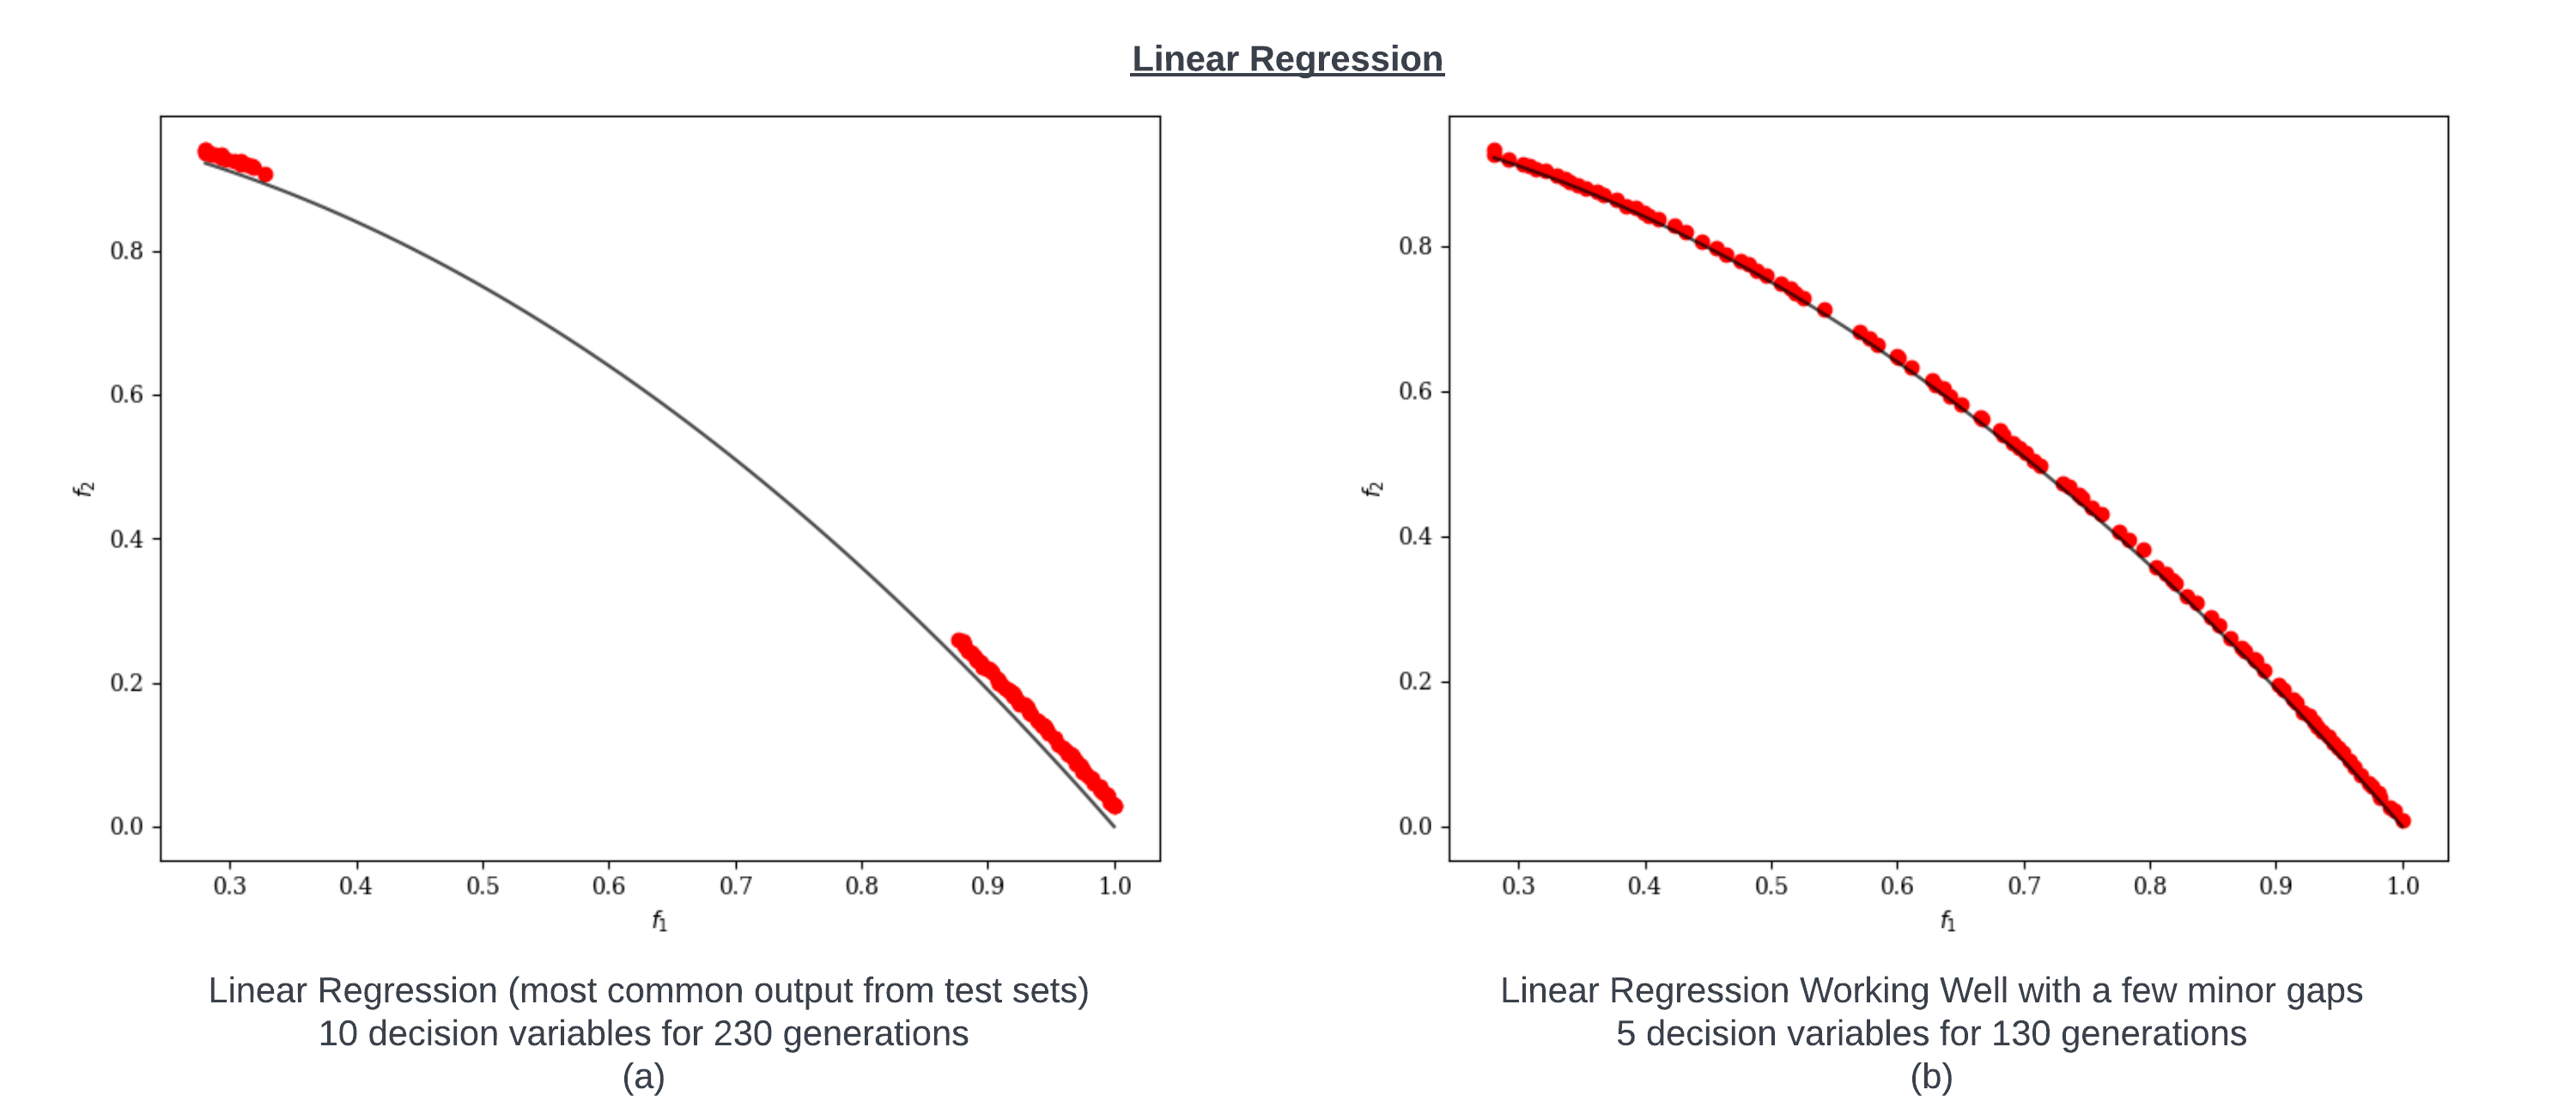
\includegraphics[width=1\linewidth]{Images/LinearRegression.png}
    \caption{ZDT6 (Table \ref{Table1}) Linear Regression for 10 and 5 decision variables}
    \label{fig:linear-regression-two}
\end{figure}

\noindent In most of the tests, as seen in figure \ref{fig:linear-regression-two}a this was the general result, often it would get stuck to one side of the Pareto front resulting in a coverage of only a small segment. This likely occurs due to it reinforcing due to the regression technique fitting a linear line between all found points, all the test sets are have non-linear Pareto fronts. As such, what ends up happening is that it either fits itself to one extreme acting similar to a tangent or two where most of it is in front or behind the Pareto front what then pushes solutions to extremes either end. \\

\noindent During testing it was found that once it converges upon an extreme, the EA pushes itself slows towards more extreme sets of solutions with a progressive lowering of diversity. This in part is due to how this the EA works in the \textit{pymoo} library with no active recall to the best previous solution (as it does not calculate overall hypervolume instead works on a selection and rejection process for the population based upon the hybrid HVC and model predictions. \\

\noindent Linear regression fits well to \textit{ZDT6} as shown in figure \ref{fig:linear-regression-two}b and for 30 decision variables overall it performs decently compared to how it usually performs. This likely occurs on \textit{ZDT6} especially as there is such a small change in the gradient as such a linear line could be fit close to it. 



\subsection{Random Forrest}

\begin{figure}[H]
    \centering
    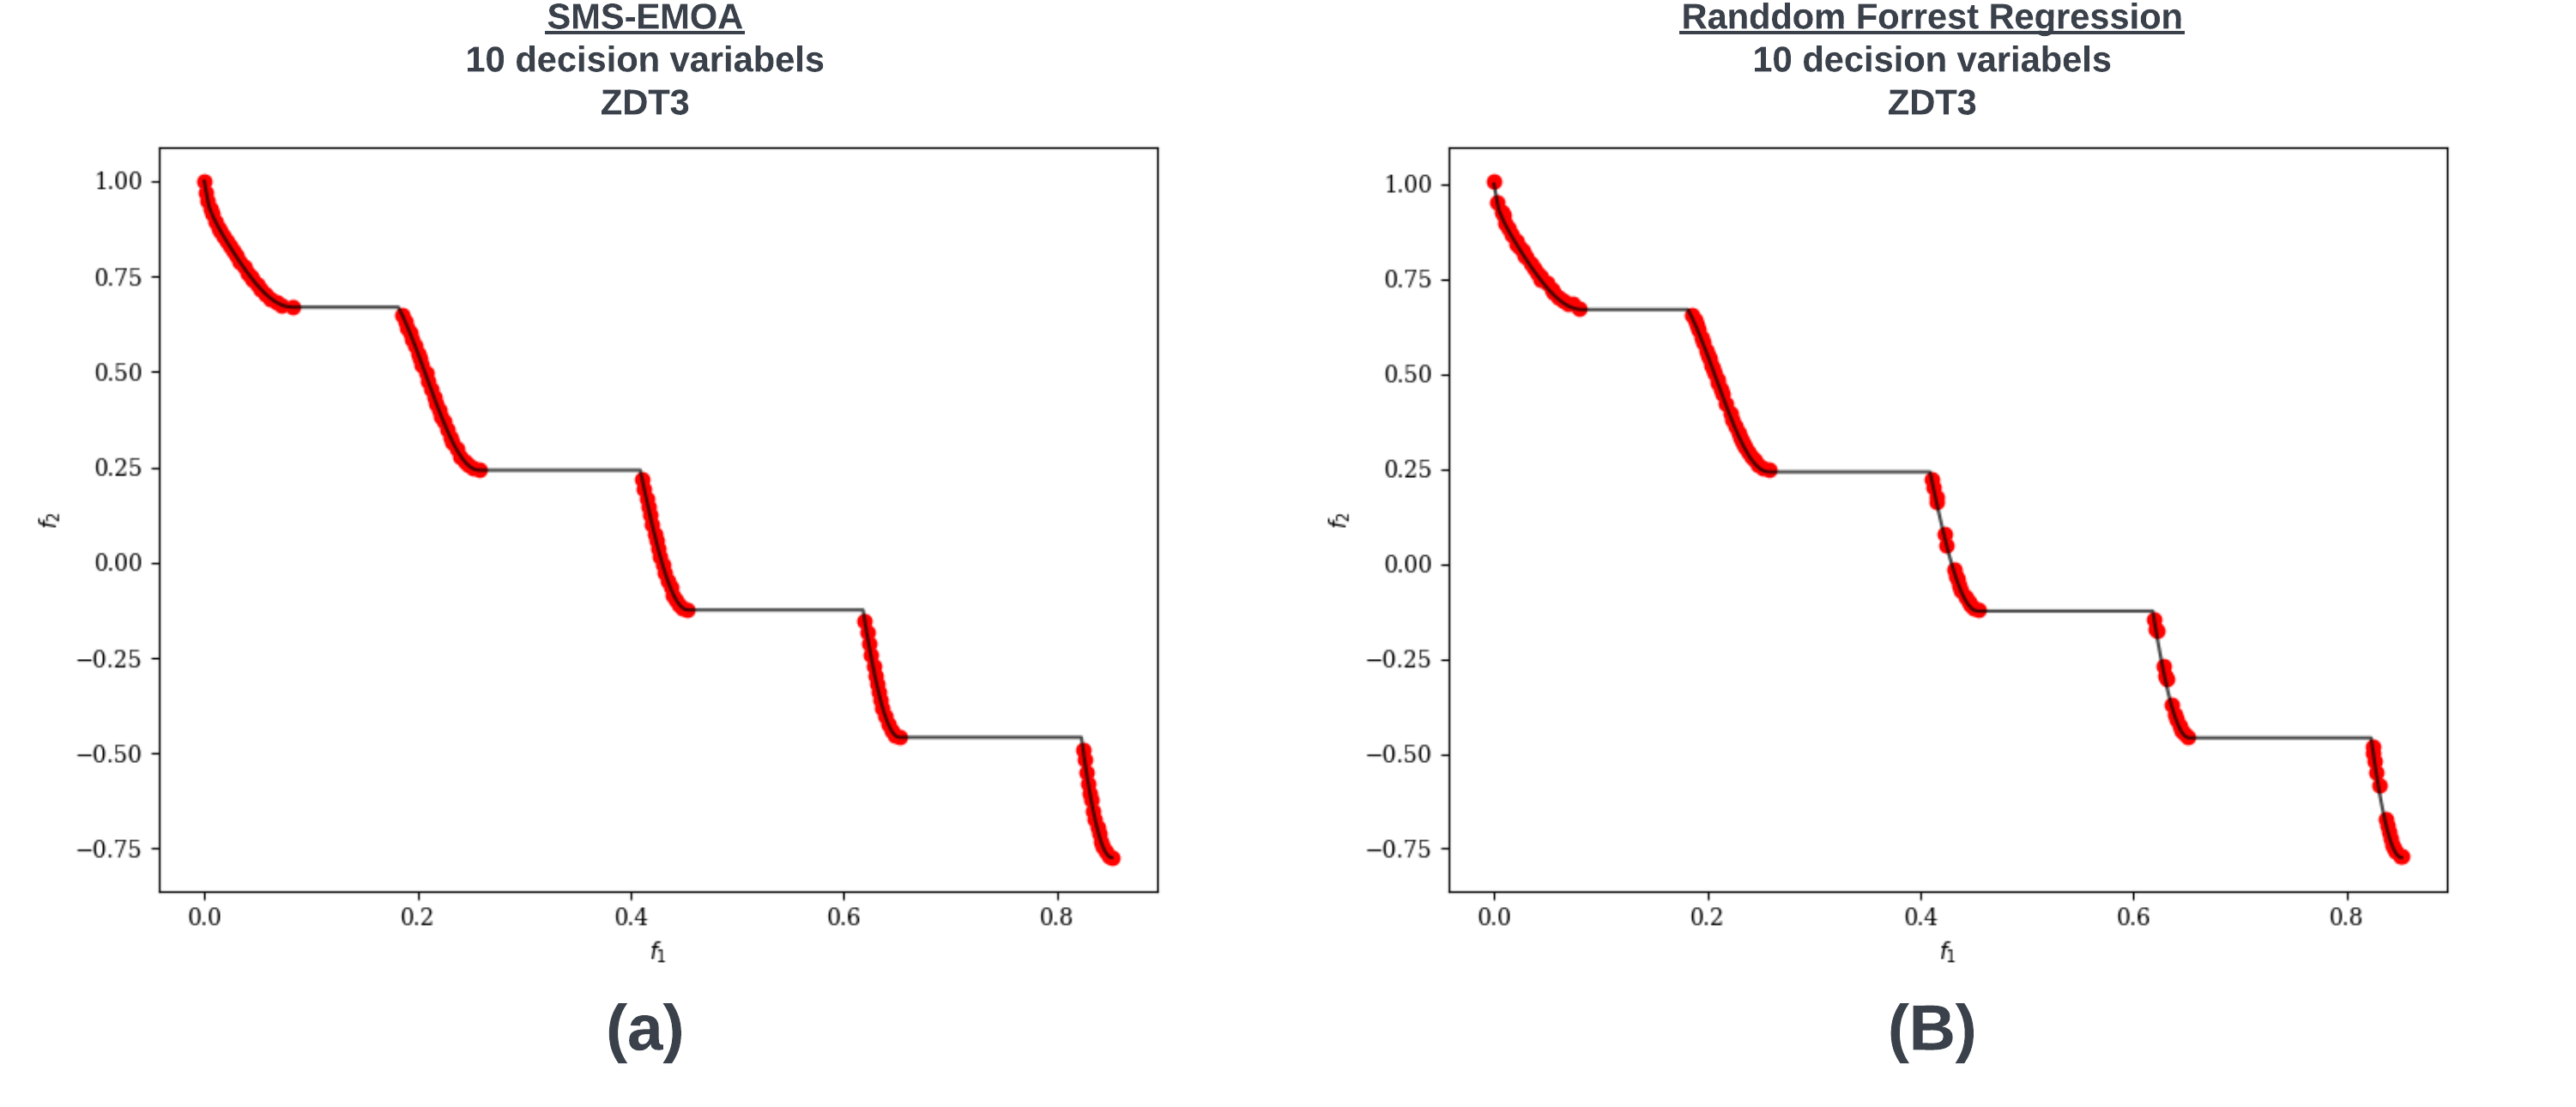
\includegraphics[width=1\linewidth]{Images/SMS_vs_RF.png}
    \caption{Random Forrest in one of the few cases it performs well}
    \label{fig:rf}
\end{figure}

Figure \ref{fig:rf} shows the RF, it performs really well on highest two steps and performs worst on the 3rd and 4th one down and only has a minor gap in the middle of the final lowest step. \\ 

\noindent Overall RF performs very well on all sets for 10 decision variables and much worse on 5 and 30. 




























\subsection{Support Vector Regression (SVR): the best for modelling hypervolume (found*)}

\begin{figure}[h]
    \centering
    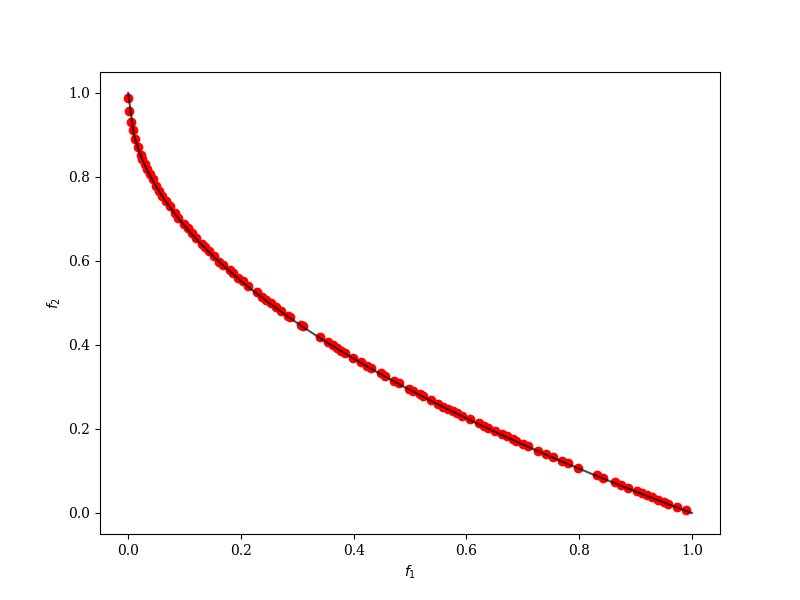
\includegraphics[width=0.7\linewidth]{Images/zvr-polykernal_1.png}
    \caption{Illustrates Support Vector Regression with the poly kernal \textit{sklearn}}
    \label{fig:svr-poly}
\end{figure}

\textbf{Support Vector Regression (SVR)} works incredibly well for all test sets excluding \textit{ZDT4}. In these three of these cases all performing better than Random Forrest. Throughout all of the solutions produced using SVR (kernal Poly or RBF) are generally well distributed along the fronts (or section of the front in the case \textit{ZDT4}). \\

\noindent In figure \ref{fig:svr-poly} it can be seen that it generally finds the front and has a good distribution across it with only two small points where there is not the greatest diversity, however comparing this is using $44.12\%$ of the original calls for calculating HVC, this should be considered very good and even matches 0.9964 (pretty much within 0.36\% similarity to the overall hypervolume of the original SMS-EMOA model for the same number of generations). \\

Why is SVR working so well to model and learn the space based on previous hypervolume contribution calculations? Well this is likely because SVR creates support vectors in the space and can then use them to guide the regression line across these points. Using the kernels RFB or Poly (degree of 3 here is set so up to (so a cubic relationship is drawn)) allow for these points to map a non-linear regression line.

\begin{figure}[H]
    \centering
    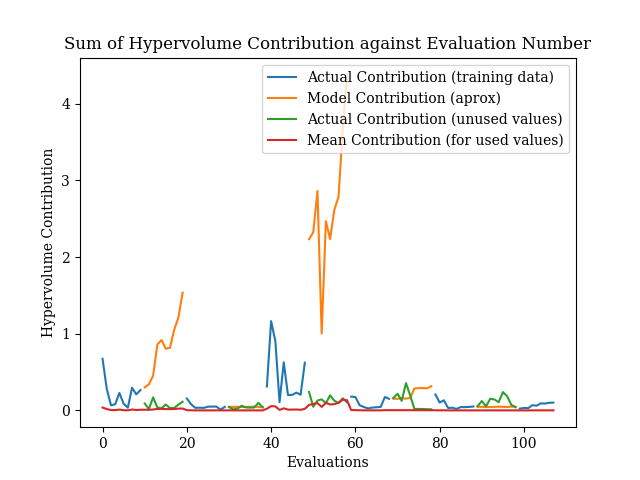
\includegraphics[width=0.7\linewidth]{Images/Figure_1_SVRPoly_ZDT1_10_graph.png}
    \caption{A continuation of the previous figure \ref{fig:svr-poly} showing the Sum of the Hypervolume Contribution (for any given set of Evaluations)}
    \label{fig:SVR-2}
\end{figure}

In the figure above this highlights some interesting, this shows that the zdt1 for 10 decision variables (Table \ref{Table1} and fig \ref{fig:svr-poly} / \ref{fig:SVR-2}) has some issues with modelling this data at certain points, ultimately this could potentially introduce some error but at these points the model is still improving this therefore suggests that where it continues on from the training set (seen in blue) the model is over predicting massively - these over predictions as they are only used as selection criteria does not seem to have a major effect on the results.  \\ 

The first model prediction set (orange) occurs most of the time, and this is likely due to the dataset chaining so much during its set of 10 predictions as such it starts over predicting when its converging. The remainder of the set where it is not over predicting, other than it progressively gets closer to the mean contribution, suggesting that as it begins to settle along Pareto front the distribution is getting better. \\ 

\section{Conclusion}

In conclusion SVR using either the Poly or the RBF kernal perform best for mimicking the Pareto front found through training on hypervolume contribution data while the EA is exploring the area. If you have 10 decision variables RF appears to be the way to go as it got pretty good at modelling the contribution for those. \\

\noindent Overall the reduction is generally very good and tends towards $50\%$ (this is likely because the \textit{pymoo} implantation does not call the survival function every generation this can only be assumed to be due to a generation being too small?) but for the tests often fall more towards $45\%$

\bibliographystyle{ACM-Reference-Format}
\bibliography{references} 

\centering

\begin{table*}[b] 
\caption{Performance Against unaltered SMS-EMOA \textit{pymoo} \& \textit{sklearn}}
\begin{tabular}{l|llllll|l|l}
\label{Table1}
 & & Decision & & Final\ \ \ \ (4.s.f) & Actual & Potential & Similarity (1) & call \\ 
Regression Model & Test Set & vars & Generations & Hypervolume  & eval calls & eval calls &  (4.s.f) & reduction (4.s.f) \\ \hline
Random Forest & ZDT1 & 5 & 40 & 0.7822 & 20 & 37 & 0.8985 & 45.95\% \\
 & & 10 & 70 & 0.8667 & 38 & 68 & 0.9961 & 44.12\% \\
 & & 30 & 140 & 0.8463 & 70 & 136 & 0.9764 & 48.53\% \\
 & ZDT3 & 5 & 40 & 1.2326 & 20 & 37 & 0.9289 & 45.95\% \\
 & & 10 & 70 & 1.3228 & 39 & 69 & 0.9982 & 43.48\% \\
 & & 30 & 120 & 1.2948 & 60 & 116 & 0.986 & 48.28\% \\
 & ZDT4 & 5 & 130 & 0.773 & 65 & 125 & 0.8874 & 48.00\% \\
 & & 10 & 190 & 0.8049 & 91 & 181 & 0.9326 & 49.72\% \\
 & & 30 & 670 & 0.829 & 309 & 609 & 0.9743 & 49.26\% \\
 & ZDT6 & 5 & 130 & 0.4908 & 64 & 124 & 0.9896 & 48.39\% \\
 & & 10 & 230 & 0.4854 & 114 & 224 & 0.99 & 49.11\% \\
 & & 30 & 600 & 0.4721 & 300 & 595 & 0.9638 & 49.58\% \\ \hline
SVR & ZDT1 & 5 & 40 & 0.8653 & 20 & 39 & 0.9939 & 48.72\% \\
Kernal = Poly & & 10 & 70 & 0.869 & 39 & 69 & 0.9987 & 43.48\% \\
 & & 30 & 140 & 0.8609 & 70 & 137 & 0.9933 & 48.91\% \\
 & ZDT3 & 5 & 40 & 1.215 & 20 & 36 & 0.9156 & 44.44\% \\
 & & 10 & 70 & 1.3218 & 39 & 69 & 0.9975 & 43.48\% \\
 & & 30 & 120 & 1.3075 & 60 & 116 & 0.9956 & 48.28\% \\
 & ZDT4 & 5 & 130 & 0.8203 & 67 & 127 & 0.9416 & 47.24\% \\
 & & 10 & 190 & 0.8054 & 91 & 181 & 0.9332 & 49.72\% \\
 & & 30 & 670 & 0.8196 & 320 & 632 & 0.9633 & 49.37\% \\
 & ZDT6 & 5 & 130 & 0.4955 & 67 & 127 & 0.999 & 47.24\% \\
 & & 10 & 230 & 0.4869 & 112 & 222 & 0.993 & 49.55\% \\
 & & 30 & 600 & 0.4877 & 293 & 583 & 0.9957 & 49.74\% \\ \hline
SVR & ZDT1 & 5 & 40 & 0.8649 & 20 & 39 & 0.9935 & 48.72\% \\ 
Kernal = RBF & & 10 & 70 & 0.8684 & 39 & 69 & 0.9981 & 43.48\% \\
 & & 30 & 140 & 0.8609 & 70 & 137 & 0.9933 & 48.91\% \\
 & ZDT3 & 5 & 40 & 1.2364 & 20 & 35 & 0.9318 & 42.86\% \\
 & & 10 & 70 & 1.3238 & 39 & 69 & 0.999* & 43.48\% \\
 & & 30 & 120 & 1.3109 & 60 & 119 & 0.9982 & 49.58\% \\
 & ZDT4 & 5 & 130 & 0.8203 & 67 & 127 & 0.9416 & 47.24\% \\
 & & 10 & 190 & 0.82 & 91 & 181 & 0.9501 & 49.72\% \\
 & & 30 & 670 & 0.8411 & 320 & 631 & 0.9886 & 49.29\% \\
 & ZDT6 & 5 & 130 & 0.495 & 66 & 126 & 0.998 & 47.62\% \\
 & & 10 & 230 & 0.4806 & 110 & 216 & 0.9803 & 49.07\% \\
 & & 30 & 600 & 0.4834 & 294 & 584 & 0.9869 & 49.66\% \\ \hline
Linear & ZDT6 & 5 & 130 & 0.4978 & 67 & 127 & 1.0037 & 47.24\% \\
 & & 10 & 230 & 0.3385 & 110 & 220 & 0.6903 & 50.0\% \\
 & & 30 & 600 & 0.4832 & 298 & 588 & 0.9866 & 49.32\% \\
\end{tabular} 
\end{table*}


\end{document}
